% OCM Dataset Integration — LaTeX Beamer Presentation
% Compile with: pdflatex ocm_presentation.tex
% Requires: beamer, booktabs, graphicx, xcolor, tikz, fontenc, inputenc

\documentclass[aspectratio=169,12pt]{beamer}

% ── Theme & Colours ────────────────────────────────────────────────────────────
\usetheme{default}
\usecolortheme{default}

\definecolor{navyblue}{RGB}{15,30,66}
\definecolor{accent}{RGB}{0,120,200}
\definecolor{lightgray}{RGB}{245,246,248}
\definecolor{darkgray}{RGB}{80,90,110}
\definecolor{green}{RGB}{16,185,129}
\definecolor{red}{RGB}{220,60,60}
\definecolor{amber}{RGB}{245,158,11}

\setbeamercolor{frametitle}{bg=navyblue, fg=white}
\setbeamercolor{title}{fg=white}
\setbeamercolor{subtitle}{fg=white!80}
\setbeamercolor{author}{fg=white!90}
\setbeamercolor{date}{fg=white!70}
\setbeamercolor{institute}{fg=white!80}
\setbeamercolor{structure}{fg=accent}
\setbeamercolor{normal text}{fg=navyblue}
\setbeamercolor{block title}{bg=accent, fg=white}
\setbeamercolor{block body}{bg=lightgray}
\setbeamercolor{alerted text}{fg=accent}
\setbeamercolor{background canvas}{bg=white}

\setbeamerfont{frametitle}{size=\large, series=\bfseries}
\setbeamerfont{title}{size=\LARGE, series=\bfseries}
\setbeamerfont{subtitle}{size=\normalsize}

% Remove navigation symbols
\setbeamertemplate{navigation symbols}{}

% Custom footline
\setbeamertemplate{footline}{%
  \leavevmode
  \hbox{%
    \begin{beamercolorbox}[wd=\paperwidth,ht=2.4ex,dp=1ex,leftskip=4mm,rightskip=4mm]{frametitle}%
      \color{white!70}\footnotesize
      OCM Dataset Integration \hfill
      \insertframenumber{} / \inserttotalframenumber
    \end{beamercolorbox}%
  }%
}

% Title page: full navy background
\setbeamertemplate{title page}{%
  \begin{tikzpicture}[remember picture, overlay]
    \fill[navyblue] (current page.south west) rectangle (current page.north east);
    \node[anchor=center] at (current page.center) {%
      \begin{minipage}{0.85\paperwidth}
        \centering
        \color{white!60}\small JAIST — Taniike Lab\par\vspace{6pt}
        {\usebeamerfont{title}\usebeamercolor[fg]{title}\inserttitle}\par\vspace{8pt}
        {\usebeamerfont{subtitle}\usebeamercolor[fg]{subtitle}\insertsubtitle}\par\vspace{20pt}
        \color{white!50}\rule{0.4\paperwidth}{0.4pt}\par\vspace{12pt}
        {\usebeamerfont{author}\usebeamercolor[fg]{author}\insertauthor}\par\vspace{4pt}
        {\small\usebeamercolor[fg]{date}\insertdate}
      \end{minipage}
    };
  \end{tikzpicture}%
}

% ── Packages ───────────────────────────────────────────────────────────────────
\usepackage[T1]{fontenc}
\usepackage[utf8]{inputenc}
\usepackage{booktabs}
\usepackage{graphicx}
\usepackage{tikz}
\usetikzlibrary{arrows.meta, positioning, shapes.geometric, fit, backgrounds}
\usepackage{array}
\usepackage{colortbl}
\usepackage{tabularx}
\usepackage{multirow}
\usepackage{amsmath}

% Convenience: coloured badge
\newcommand{\badge}[2]{%
  \colorbox{#1}{\color{white}\footnotesize\bfseries\,#2\,}}

% ── Meta ───────────────────────────────────────────────────────────────────────
\title{Integrating OCM Literature Data\\into Lab-Scale ML Models}
\subtitle{Domain-Adaptive Transfer Learning for Catalyst Yield Prediction}
\author{Partha Nupam Nagar}
\date{May 2026}
\institute{JAIST — Taniike Lab}

% ══════════════════════════════════════════════════════════════════════════════
\begin{document}
% ══════════════════════════════════════════════════════════════════════════════

% ── Slide 1 — Title ────────────────────────────────────────────────────────────
\begin{frame}[plain]
  \titlepage
\end{frame}

% ── Slide 2 — Two Datasets ────────────────────────────────────────────────────
\begin{frame}{Two Very Different Datasets}

  \begin{columns}[T]

    \begin{column}{0.47\textwidth}
      \begin{block}{Our Lab Data (Internal)}
        \begin{tabular}{ll}
          \toprule
          \textbf{Samples}      & 89{,}074 \\
          \textbf{Year}         & 2025 \\
          \textbf{Preparation}  & Impregnation only \\
          \textbf{Mean Y(C2)}   & 5.25\% \\
          \textbf{Conditions}   & Controlled \\
          \bottomrule
        \end{tabular}
        \vspace{4pt}

        \badge{accent}{Strength} High volume, consistent protocol\\[4pt]
        \badge{red}{Gap} Narrow chemical diversity
      \end{block}
    \end{column}

    \begin{column}{0.47\textwidth}
      \begin{block}{Literature Data (Public, $\leq$ 2019)}
        \begin{tabular}{ll}
          \toprule
          \textbf{Samples}      & 3{,}852 \\
          \textbf{Year}         & 1982–2019 \\
          \textbf{Preparation}  & 15+ methods \\
          \textbf{Mean Y(C2)}   & 8.67\% \\
          \textbf{Conditions}   & Mixed labs \\
          \bottomrule
        \end{tabular}
        \vspace{4pt}

        \badge{green}{Strength} Chemical diversity, high-yield recipes\\[4pt]
        \badge{red}{Gap} Publication bias, missing conditions
      \end{block}
    \end{column}

  \end{columns}

  \vspace{8pt}
  \centering
  \colorbox{lightgray}{\parbox{0.9\textwidth}{\centering\small
    \textbf{Challenge:} $\Delta\overline{Y}(\text{C}_2) = 8.67 - 5.25 = \mathbf{3.42\%}$\ \
    ($t = -32.2$, $p = 2.3 \times 10^{-202}$) — datasets are statistically different
  }}

\end{frame}

% ── Slide 3 — Domain Gap ──────────────────────────────────────────────────────
\begin{frame}{Domain Gap: Why We Cannot Just Mix the Data}

  \begin{columns}[T]

    \begin{column}{0.48\textwidth}
      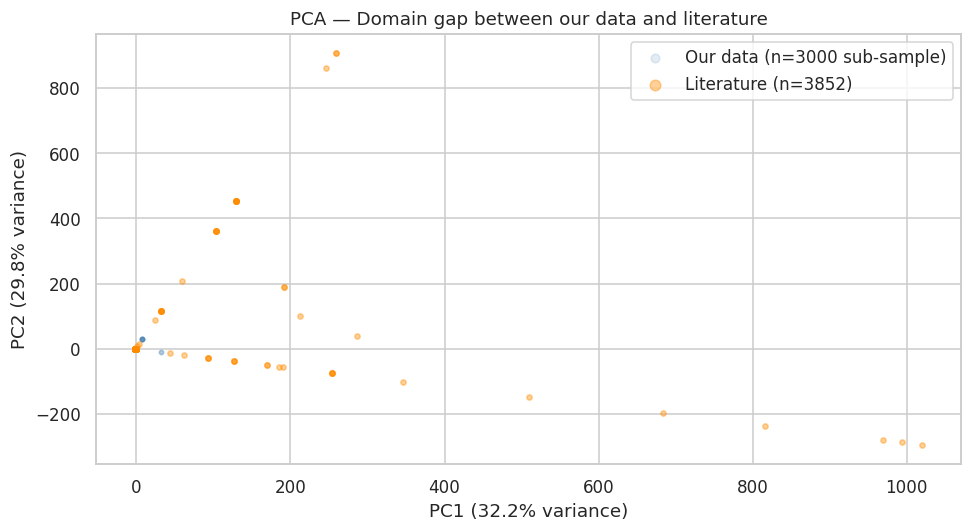
\includegraphics[width=\linewidth]{fig_pca_domain_gap.png}
    \end{column}

    \begin{column}{0.48\textwidth}
      \vspace{6pt}
      \textbf{What the PCA shows}
      \begin{itemize}
        \item 65 element features compressed to 2D
        \item \textcolor{accent}{Blue} = our lab (89k); \textcolor{red}{Red} = literature (3.8k)
        \item Literature spans regions our model has never seen
      \end{itemize}

      \vspace{10pt}
      \textbf{Key facts}
      \begin{itemize}
        \item \badge{red}{78.5\%} of literature samples are out-of-distribution
        \item Ba dominates our data; Si/Na/Mn dominate literature
        \item 15+ preparation methods vs.\ our single protocol
      \end{itemize}

      \vspace{10pt}
      \colorbox{lightgray}{\parbox{\linewidth}{\small
        \textbf{Naive concatenation inflates} training error and introduces
        systematic bias: literature samples vote equally despite
        representing a different measurement regime.
      }}
    \end{column}

  \end{columns}

\end{frame}

% ── Slide 4 — Methods & RMSE Table ────────────────────────────────────────────
\begin{frame}{Five Approaches to Selective Transfer}

  \renewcommand{\arraystretch}{1.3}
  \begin{tabularx}{\textwidth}{lX r r}
    \toprule
    \textbf{Method} & \textbf{Core Idea} & \textbf{CV RMSE} & \textbf{$\Delta$} \\
    \midrule
    Baseline (no lit.) & LightGBM on lab data only & 2.133 & — \\
    \rowcolor{lightgray}
    Naive concat. & Add all literature rows & 2.248 & \textcolor{red}{$+5.4\%$} \\
    DRST ($\tau=0.30$) & Keep 782 similar lit.\ samples & 2.019 & \textcolor{darkgray}{$-5.3\%$} \\
    KMM weights & Soft per-sample importance & 2.035 & \textcolor{darkgray}{$-4.6\%$} \\
    Bias correction & Quantile-normalise Y(C2) & 2.044 & \textcolor{darkgray}{$-4.2\%$} \\
    \rowcolor{green!15}
    \textbf{Two-stage (Dir.\ A)} & \textbf{XGBoost prior + DRST} & \textbf{1.907} & \textcolor{green}{\textbf{$-10.6\%$}} \\
    \bottomrule
  \end{tabularx}

  \vspace{8pt}
  \small
  \textbf{OOD test} (2,139 held-out literature samples, never trained on):\\
  Baseline $6.53$ $\rightarrow$ Two-stage $3.60$ \quad \badge{green}{$-\mathbf{45\%}$}

\end{frame}

% ── Slide 5 — Two-Stage Pipeline ──────────────────────────────────────────────
\begin{frame}{Two-Stage Fine-Tuning Pipeline}

  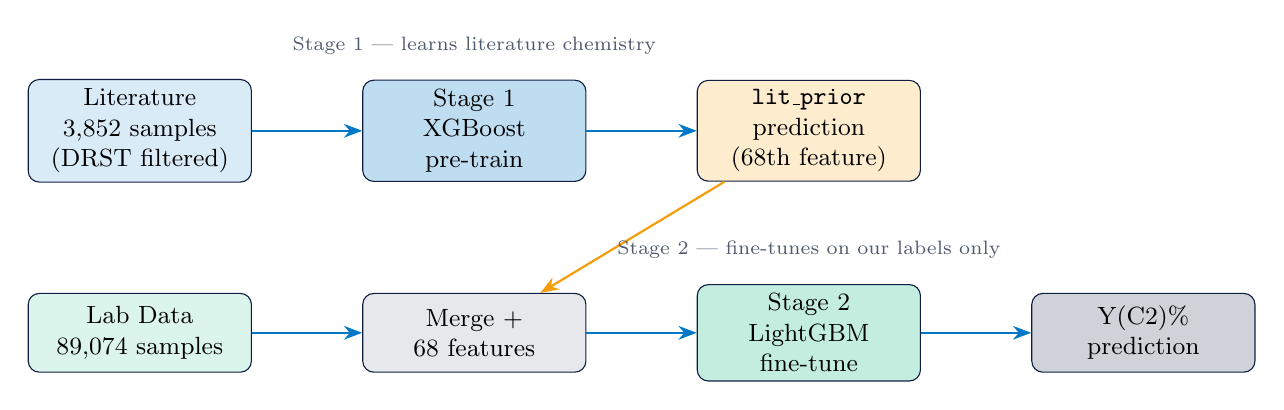
\begin{tikzpicture}[
      box/.style={rectangle, rounded corners=4pt, draw=navyblue, fill=lightgray,
                  text width=2.6cm, align=center, minimum height=1.0cm, font=\small},
      arrow/.style={-{Stealth}, thick, color=accent},
      label/.style={font=\scriptsize, color=darkgray},
      every node/.style={font=\small}
    ]

    % Stage 1
    \node[box, fill=accent!15] (lit) {Literature\\3,852 samples\\(DRST filtered)};
    \node[box, right=1.4cm of lit, fill=accent!25] (xgb) {Stage 1\\XGBoost\\pre-train};
    \node[box, right=1.4cm of xgb, fill=amber!20] (prior) {\texttt{lit\_prior}\\prediction\\(68th feature)};

    \draw[arrow] (lit) -- (xgb);
    \draw[arrow] (xgb) -- (prior);

    % Stage 2
    \node[box, below=1.4cm of lit, fill=green!15] (lab) {Lab Data\\89,074 samples};
    \node[box, right=1.4cm of lab, fill=navyblue!10] (merge) {Merge +\\68 features};
    \node[box, right=1.4cm of merge, fill=green!25] (lgbm) {Stage 2\\LightGBM\\fine-tune};
    \node[box, right=1.4cm of lgbm, fill=navyblue!20] (out) {Y(C2)\%\\prediction};

    \draw[arrow] (lab) -- (merge);
    \draw[arrow] (merge) -- (lgbm);
    \draw[arrow] (lgbm) -- (out);

    % Cross arrow from prior to merge
    \draw[arrow, color=amber] (prior) -- (merge);

    % Stage labels
    \node[label, above=0.2cm of xgb] {Stage 1 — learns literature chemistry};
    \node[label, above=0.2cm of lgbm] {Stage 2 — fine-tunes on our labels only};

  \end{tikzpicture}

  \vspace{6pt}
  \small
  \textbf{Key property:} Stage 2 trains \emph{only on internal labels} — literature biases
  cannot directly corrupt the final model.\ The prior acts as a soft regulariser,
  not a supervisor.

\end{frame}

% ── Slide 6 — Results ─────────────────────────────────────────────────────────
\begin{frame}{Results at a Glance}

  \begin{columns}[T]

    \begin{column}{0.52\textwidth}
      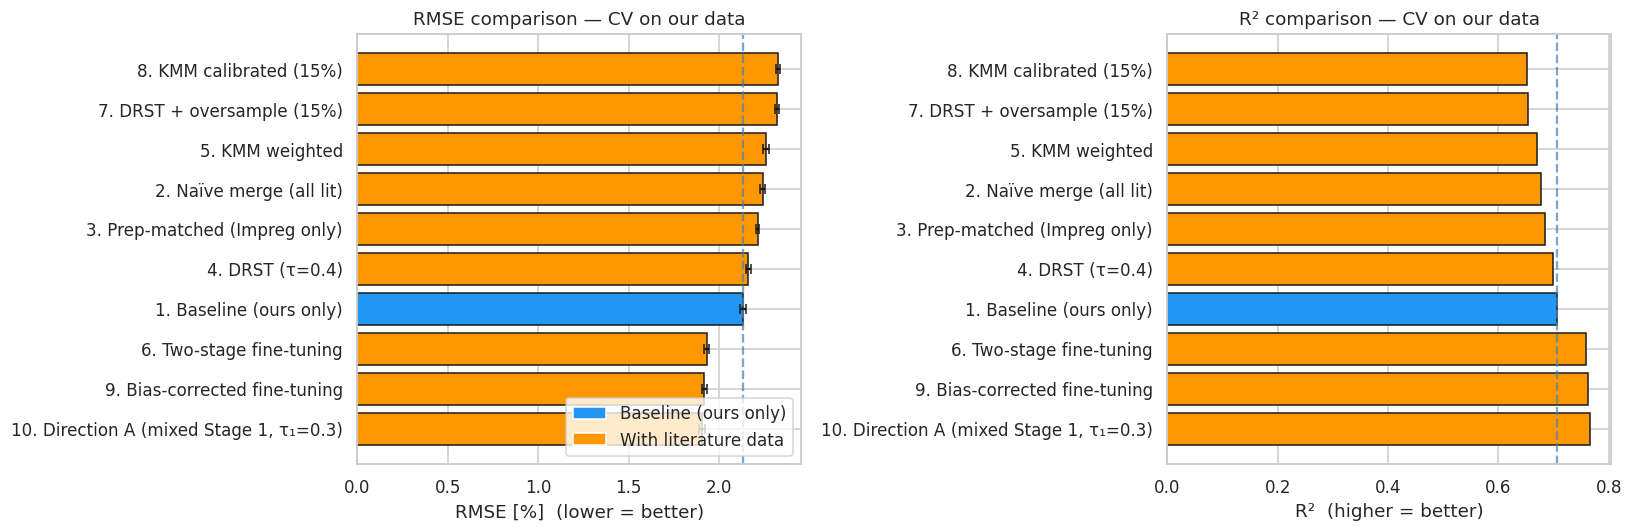
\includegraphics[width=\linewidth]{fig_results_comparison.png}
    \end{column}

    \begin{column}{0.44\textwidth}
      \vspace{4pt}
      \textbf{Cross-validated RMSE (5-fold, asymmetric)}

      \vspace{6pt}
      \begin{tabular}{lc}
        \toprule
        & RMSE (\%) \\
        \midrule
        Baseline & 2.133 \\
        \textbf{Two-stage} & \textbf{1.907} \\
        Improvement & \badge{green}{$-10.6\%$} \\
        \bottomrule
      \end{tabular}

      \vspace{12pt}
      \textbf{OOD Robustness (held-out literature)}

      \vspace{6pt}
      \begin{tabular}{lc}
        \toprule
        & RMSE (\%) \\
        \midrule
        Baseline & 6.53 \\
        \textbf{Two-stage} & \textbf{3.60} \\
        Improvement & \badge{green}{$-45\%$} \\
        \bottomrule
      \end{tabular}

      \vspace{10pt}
      \colorbox{lightgray}{\parbox{\linewidth}{\scriptsize
        OOD: 2,139 samples from non-Impregnation
        literature methods, never seen during training.
      }}
    \end{column}

  \end{columns}

\end{frame}

% ── Slide 7 — SHAP Analysis ───────────────────────────────────────────────────
\begin{frame}{What Drives the Model? (SHAP Analysis)}

  \begin{columns}[T]

    \begin{column}{0.50\textwidth}
      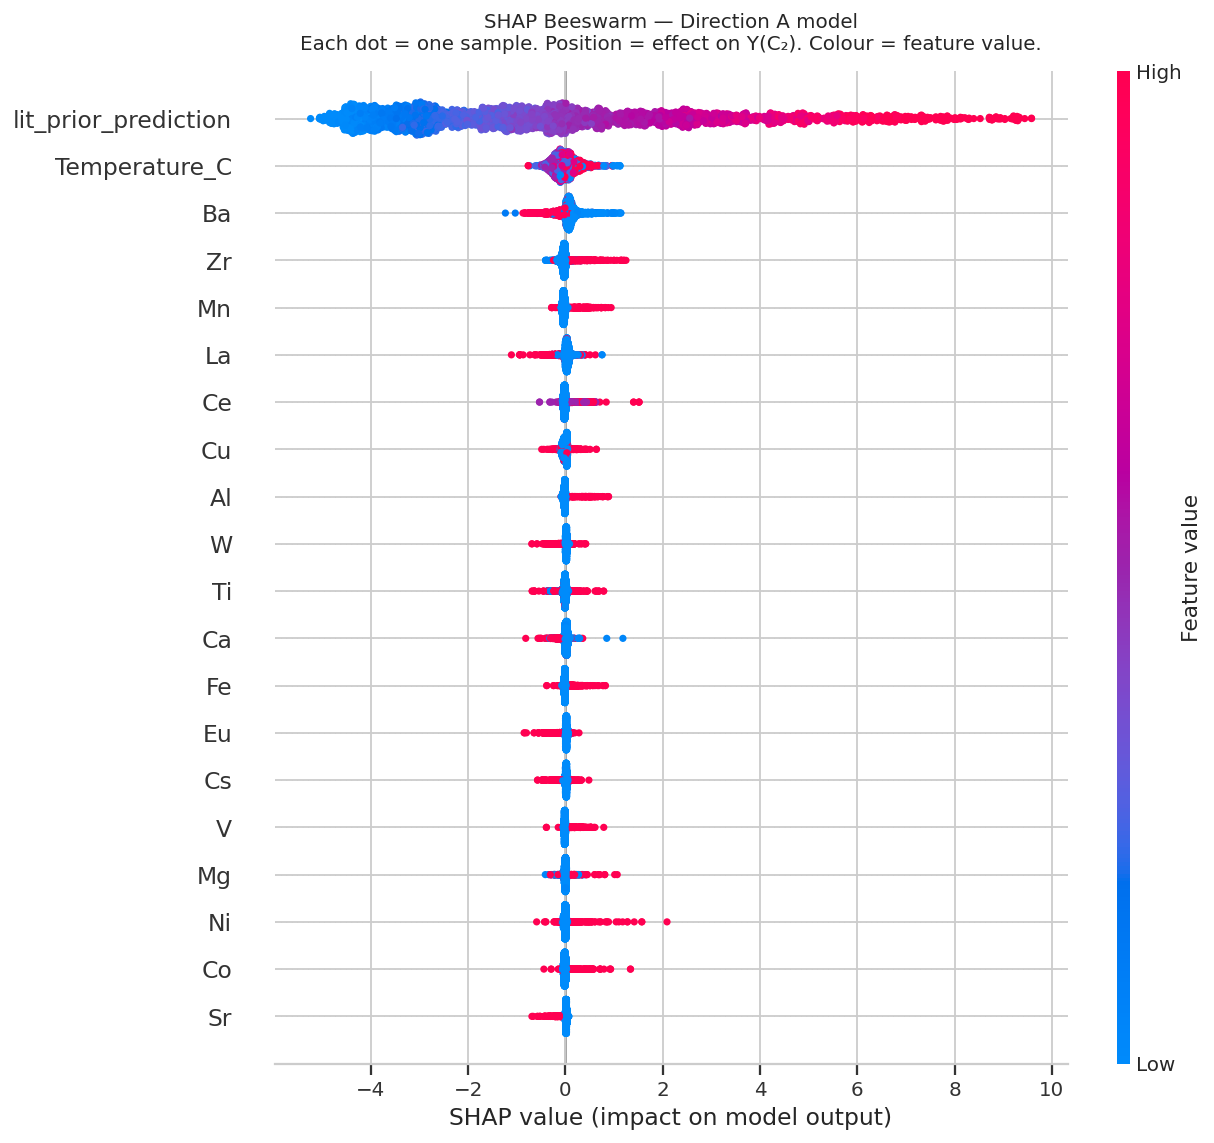
\includegraphics[width=\linewidth]{fig_shap_beeswarm.png}
    \end{column}

    \begin{column}{0.46\textwidth}
      \vspace{4pt}
      \textbf{Top findings (3,000 sample subsample)}
      \begin{itemize}
        \item \textbf{\#1 feature:} \texttt{lit\_prior\_prediction} — literature chemistry knowledge is actively used
        \item \textbf{Temperature} — strong positive; higher $T$ favours C2
        \item \textbf{Ba, Mn, La, Ce} — all raise predicted yield
        \item \textbf{Li, K} — mixed / suppressive effect
      \end{itemize}

      \vspace{8pt}
      \textbf{Residual pattern (ceiling effect)}
      \begin{tabular}{lc}
        \toprule
        Y(C2) range & RMSE \\
        \midrule
        0–6\%   & 1.43–1.48 \\
        6–10\%  & 1.95 \\
        10–15\% & 2.58 \\
        $>$15\% & 4.70 \quad \badge{red}{$-4.2\%$ bias} \\
        \bottomrule
      \end{tabular}

      \vspace{6pt}
      \scriptsize Root cause: GHSV, CH$_4$/O$_2$ ratio, and pressure
      are absent from the dataset.
    \end{column}

  \end{columns}

\end{frame}

% ── Slide 8 — Limitations & Next Steps ────────────────────────────────────────
\begin{frame}{Limitations \& Next Steps}

  \begin{columns}[T]

    \begin{column}{0.32\textwidth}
      \begin{block}{Option A — \badge{green}{Easy}}
        \textbf{Add reaction conditions}\\[4pt]
        \small
        Include GHSV, CH$_4$/O$_2$, pressure as features.\\[4pt]
        Expected to fix the $>$15\% ceiling effect and reduce high-yield RMSE from 4.70 to $\sim$2.5.
      \end{block}
    \end{column}

    \begin{column}{0.32\textwidth}
      \begin{block}{Option B — \badge{amber}{Medium}}
        \textbf{Tune transfer threshold}\\[4pt]
        \small
        Sweep DRST $\tau$ and Stage 1 sample size jointly.\\[4pt]
        Current best: $\tau=0.30$ (782 samples).\ Grid search may recover 0.3–0.5\% RMSE.
      \end{block}
    \end{column}

    \begin{column}{0.32\textwidth}
      \begin{block}{Option C — \badge{red}{Hard}}
        \textbf{Neural domain adaptation}\\[4pt]
        \small
        Replace LightGBM with domain-adversarial NN (DANN) or CORAL.\\[4pt]
        High complexity; justifiable only after reaction conditions are added.
      \end{block}
    \end{column}

  \end{columns}

  \vspace{10pt}
  \begin{columns}[T]
    \begin{column}{0.48\textwidth}
      \textbf{Key Limitations}
      \begin{itemize}
        \item Missing GHSV / CH$_4$:O$_2$ / pressure features
        \item Literature has 15+ prep methods — coverage uneven
        \item Publication bias: only successful experiments published
        \item OOD improvement may not generalise to new catalyst families
      \end{itemize}
    \end{column}
    \begin{column}{0.48\textwidth}
      \textbf{Recommended Priority}
      \begin{enumerate}
        \item Collect and add GHSV + CH$_4$/O$_2$ \badge{green}{highest impact}
        \item Re-run two-stage with expanded feature set
        \item Revisit $\tau$ tuning with updated data
      \end{enumerate}
    \end{column}
  \end{columns}

\end{frame}

% ══════════════════════════════════════════════════════════════════════════════
\end{document}
